\documentclass[
   12pt,
   headsepline=0pt,
   ngerman,
   a4paper,
   oneside,
   titlepage,
   parskip=full,
   listof=totoc,
   bibliography=totoc,
   index=totoc,
   final,
   numbers=noenddot
]{scrartcl}

% !TEX root = ../Grunddatei.tex
%Wenn die Texte Umlaute oder ein Esszet enthalten, muss der folgende           Befehl bereits an dieser Stelle aktiviert werden:            %\usepackage[latin1]{inputenc}

\newcommand{\art}{Bachelorarbeit}
\newcommand{\titel}{Entwurf einer erweiterbaren Softwarearchitektur im Inbetriebnahmemanagement unter
Nutzung des IFC-Standards}
\newcommand{\untertitel}{}
\newcommand{\fachgebiet}{Medieninformatik}
\newcommand{\autor}{Jan Händl}
\newcommand{\studienbereich}{Informatik/Mathematik}
\newcommand{\matrikelnr}{50290}
\newcommand{\erstgutachter}{Prof. Dr. Tim Pidun}
\newcommand{\zweitgutachter}{Dipl.-Inf. Claus Engelhardt}
\newcommand{\jahr}{2026}
\newcommand{\ort}{HTW Dresden}
\newcommand{\logo}{Bilder/HTWD_logo_RGB_horizontal_color.png}
% !TEX root = ../Abschlussarbeit_Jan_Höndl.tex
\usepackage{amsmath}
\usepackage{amssymb}
\usepackage{graphicx}
\usepackage{hyperref} 
\hypersetup{
    colorlinks=true,
    linkcolor=black,    % Interne Links (Inhaltsverzeichnis etc.)
    citecolor=black,    % Zitate
    filecolor=black,
    urlcolor=black      % Web-Links
}
\usepackage{subcaption}
\captionsetup{
    font=small,              % Etwas kleiner als der Haupttext
    labelfont=bf,            % "Abbildung 1:" in fett
    labelsep=colon,          % Doppelpunkt nach der Nummer
    format=plain,            % Text bündig unter dem Label
    margin=10pt              % Einrückung links/rechts zur besseren Trennung vom Text
}

% Spezielle Konfiguration für die kleinen Unterabbildungen (falls nötig)
\captionsetup[sub]{
    font=footnotesize,       % Noch ein Stück kleiner für a), b), c)
    labelfont=md             % Label hier nicht fett, sondern normal
}
\usepackage{here}
\usepackage{color}
\usepackage{textcomp}
\usepackage{pdfpages}
\usepackage{multirow}
\usepackage{microtype}


%Zeilenabstände und Seitenränder
\usepackage{setspace}
\singlespacing
\usepackage{geometry}
\geometry{
  a4paper,
  left=40mm,           % Linker Rand (Bindung)
  right=20mm,          % Rechter Rand
  top=30mm,            % Oberer Rand
  bottom=30mm,         % Unterer Rand
  headsep=12.5mm,      % Abstand zu Kopfzeile (1,25 cm)
  footskip=12.5mm,     % Abstand zu Fußzeile (1,25 cm)
  includeheadfoot=false % Ränder gelten ab Blattkante
}

\graphicspath{{Bilder/}}
% Ebene 1: 16 Pkt, Fett, Linksbündig
\setkomafont{section}{\fontsize{16pt}{20pt}\selectfont\bfseries\rmfamily}

% Ebene 2: 14 Pkt, Fett, Linksbündig
\setkomafont{subsection}{\fontsize{14pt}{18pt}\selectfont\bfseries\rmfamily}

% Ebene 3: 12 Pkt, Fett, Linksbündig
\setkomafont{subsubsection}{\fontsize{12pt}{14pt}\selectfont\bfseries\rmfamily}

% Ebene 4: 12 Pkt, Kursiv, Linksbündig
% (In scrartcl ist die 4. Ebene meist \paragraph)
\setkomafont{paragraph}{\fontsize{12pt}{14pt}\selectfont\itshape}

\usepackage{scrlayer-scrpage}
\usepackage{enumitem}
% Optional: Global alle Listen kompakter machen
\setlist[itemize]{noitemsep, topsep=0pt}

\usepackage[
  backend=biber,       % Nutze Biber als Sortier-Engine (wichtig!)
  style=authoryear,    % Zitierstil (z. B. Autor-Jahr-Stil: (Feth 2023))
  % style=numeric,     % Alternativ: Numerischer Stil: [1]
]{biblatex}
\addbibresource{Bibliographie.bib}
\let\cite\parencite    % Ermöglicht geklammerte Zitate mit \cite wie bei natbib
\usepackage[ngerman]{todonotes}

%Abkürzungsbibliothek
\usepackage[printonlyused]{acronym}
%Glossar
\usepackage[automake]{glossaries}
\makeglossaries

\usepackage{fontspec}
\setmainfont{Times New Roman} % Legt Times New Roman als Hauptschriftart fest
%Code
%Siehe auch: http://ctan.ebinger.cc/tex-archive/macros/latex/contrib/listings/lstdrvrs.pdf
\usepackage{listings}
\usepackage{xcolor}
\definecolor{neo4jSpace}{HTML}{FF9F9F}       % Rosa für IfcSpace
\definecolor{neo4jStorey}{HTML}{B3A2C7}      % Lila für IfcBuildingStorey
\definecolor{neo4jBg}{HTML}{12161A}          % Dunkler Graph-Hintergrund
\definecolor{neo4jSelection}{HTML}{A5F3FC}
% Definition der Inline-Boxen für die Labels (ahmt die Neo4j-GUI nach)
%\usepackage{uarial}
\definecolor{json_key}{rgb}{0,0,0.6}
\definecolor{json_string}{rgb}{0,0.5,0}
\lstdefinelanguage{cypher}{
    morekeywords={MATCH, WHERE, RETURN, AND, NOT, OR, WITH, UNWIND, CREATE, MERGE, DELETE, SET, REMOVE},
    sensitive=true,
    morecomment=[l]{//},
    morestring=[b]",
    morestring=[b]',
}

\lstdefinelanguage{IFC}{
    morekeywords={ISO, HEADER, FILE_DESCRIPTION, FILE_NAME, FILE_SCHEMA, ENDSEC, DATA, END, IFCPROJECT, IFCOWNERHISTORY, IFCPERSONANDORGANIZATION, IFCPERSON, IFCORGANIZATION, IFCAPPLICATION, IFCUNITASSIGNMENT, IFCSIUNIT, IFCGEOMETRICREPRESENTATIONCONTEXT, IFCAXIS2PLACEMENT3D, IFCCARTESIANPOINT, IFCSITE, IFCBUILDING, IFCPOSTALADDRESS, IFCBUILDINGSTOREY, IFCWALLSTANDARDCASE, IFCLOCALPLACEMENT, IFCPRODUCTDEFINITIONSHAPE, SHAPEREPRESENTATION, EXTRUDEDAREASOLID, IFCRECTANGLEPROFILEDEF, IFCDIRECTION, IFCRELCONTAINEDINSPATIALSTRUCTURE},
    sensitive=true,
    morecomment=[s]{/*}{*/},
    morestring=[b]'
}

\lstset{
    basicstyle=\ttfamily\small,
    breaklines=true,
    numbers=left,
    numberstyle=\tiny\color{gray},
    keywordstyle=\color{blue}\bfseries,
    stringstyle=\color{orange},
    commentstyle=\color{green!60!black},
    frame=lines,
    captionpos=b
}
\lstdefinelanguage{GraphQL}{
  keywords={interface, implements, type, schema, scalar, input},
  keywordstyle=\color{blue}\bfseries,
  ndkeywords={ID, String, Int, Float, Boolean},
  ndkeywordstyle=\color{purple}\bfseries,
  identifierstyle=\color{black},
  sensitive=true,
  comment=[l]{\#},
  commentstyle=\color{gray}\ttfamily,
  stringstyle=\color{red}\ttfamily,
  morestring=[b]",
}
\lstdefinelanguage{json}{
    basicstyle=\normalfont\ttfamily\small,
    numbers=left,
    numberstyle=\scriptsize,
    stepnumber=1,
    numbersep=8pt,
    showstringspaces=false,
    breaklines=true,
    frame=lines,
    string=[s]{"}{"},
    comment=[l]{:\ },
    morecomment=[s]{"{}}{"},
}

% Globale Einstellungen für den Code-Block
\lstset{
  language=GraphQL,
  backgroundcolor=\color{gray!5},
  basicstyle=\small\ttfamily,
  breaklines=true,
  captionpos=b,
  frame=single,
  numbers=left,
  numberstyle=\tiny\color{gray},
  tabsize=2,
  showstringspaces=false
}


\usepackage{chngcntr}
\counterwithin{figure}{section}
\usepackage[perpage]{footmisc}
\usepackage[ngerman]{babel}


% !TEX root = ../Abschlussarbeit_DE.tex

% --- Seitenstil-Bereinigung und Linien-Aktivierung ---
\clearpairofpagestyles

% Aktiviert die Trennlinien für Kopf- und Fußzeile exakt nach Vorgabe
\KOMAoptions{
  headsepline=0.4pt, % Waagerechter Strich unter der Kopfzeile
}

% --- Typografie in Kopf- und Fußzeile ---
% Laut Vorgabe: Kopf-/Fußzeilentext in 10 Pkt.
\setkomafont{pageheadfoot}{\fontsize{10}{12}\selectfont\normalfont\rmfamily}
% Laut Vorgabe: Seitennummer in 12 Pkt.
\setkomafont{pagenumber}{\fontsize{12}{14}\selectfont\normalfont\rmfamily}

% --- Geometrie-Anpassung für das Logo ---
\setlength{\headheight}{21mm} % Höhe der Kopfzeile (beibehalten wegen des Logos)
% Wichtig für den Druck: Der Fließtext muss nach der Trennlinie nach unten verschoben werden
\geometry{headsep=12.5mm} 

% --- Kopfzeile Definition ---
\rohead{\includegraphics[scale=0.1]{\logo}} % Logo rechts oben
\lehead{\leftmark} % Aktueller Kapitelname links oben

% --- Fußzeile Definition ---
\ifoot{}
\cfoot{}
% Setzt die Seitenzahl nach rechts außen (sowohl auf normalen Seiten [obacht] als auch auf Kapitelseiten)
\ofoot[\pagemark]{\pagemark}



\makeindex

\begin{document}

% --- 1. DECKBLATT ---
% !TEX root = ../Grunddatei.tex

% 1. Ränder für das Deckblatt temporär ändern (z.B. alles auf 2.5cm oder nach Wunsch)
\newgeometry{left=2.5cm, right=2.5cm, top=2.5cm, bottom=2.5cm, }

\thispagestyle{plain}
\begin{titlepage}
	\setlength{\parindent}{0pt} % <--- Das hier hinzufügen!
    \begin{center}
        \vspace*{2.5 cm}
        \includegraphics[width=0.5\linewidth]{\logo}\\[1.25cm]
        \LARGE{\textbf{Bachelorarbeit}}\\[3.5ex]
		\LARGE{\textbf{\titel}}\\[3.5ex]
        \normalsize
        \begin{tabular}{p{5.4cm}p{5cm}}\\
            vorgelegt von:  & \quad \autor\\[1.2ex]
            Studienbereich: & \quad \studienbereich\\[1.2ex]
            Ort: & \quad \ort\\[1.2ex]
            Matrikelnummer: & \quad \matrikelnr\\[1.2ex]
            Erstgutachter:  & \quad \erstgutachter\\[1.2ex]
                Zeitraum:    & \quad 27.03.2026 - 16.08.2026 \\[1.2ex]
            Abgabedatum:    & \quad 16.09.2026
        \end{tabular}
        
        \vspace{2cm} % Ein bisschen Puffer nach unten
        \copyright\ \jahr\\[9ex]
    \end{center}
    
    %\singlespacing
    %\small
    %\noindent Dieses Werk einschließlich seiner Teile ist \textbf{urheberrechtlich geschützt}...
    
\end{titlepage}

% 2. Hier werden die Ränder wieder auf die Werte aus deiner Grunddatei zurückgesetzt
\restoregeometry

% --- 2. VORSPANN (Römisch & KEINE Kapitelnummern) ---
\clearpage
\pagenumbering{Roman}      % Startet I, II, III...
\setcounter{secnumdepth}{-1} % Schaltet Kapitelnummern AUS (z.B. für Abstract, Verzeichnisse)

% !TEX root = ../Abschlussarbeit_Jan_Händl.tex
\section*{Abstract}
Hier kommt noch ein abstract rein
\tableofcontents 
\clearpage

% !TEX root = ../Abschlussarbeit_Jan_Händl.tex
\section{Abkürzungsverzeichnis}
\begin{acronym}[GraphQL]
    \acro{IFC}{Industry Foundation Classes}
    \acro{BIM}{Building Information Modeling}
    \acro{REST}{Representational State Transfer}
    \acro{GraphQL}{Graph Query Language}
    \acro{PWA}{Progressive Web App}
    \acro{ERP}{Enterprise Resource Planning}
    \acro{MSR}{Mess-, Steuer- und Regelungstechnik}
    \acro{TGA}{Technische Gebäudeausrüstung}
    \acro{UI}{User Interface}
    \acro{CI/CD}{Continuous Integration/Continuous Delivery}

\end{acronym}
% !TEX root = ../Abschlussarbeit_Jan_Händl.tex
\newglossaryentry{Express}{
  name={EXPRESS},
  description={EXPRESS ist ein Standard für eine generische Datenmodellierungssprache für Produktdaten.
      EXPRESS ist im ISO-Standard für den Austausch von Produktmodelldaten STEP (ISO 10303) formalisiert und als ISO 10303-11 standardisiert}
}
\newglossaryentry{API}{
  name={API},
  description={Eine Schnittstelle, die es zwei oder mehr Programmen ermöglicht, miteinander zu kommunizieren (Application Programming Interface)}
}

\newglossaryentry{Framework}{
  name={Framework},
  description={Ein vorgefertigtes Gerüst, das die Entwicklung von Software vereinfacht}
}

\newglossaryentry{Webapplikation}{
  name={Webanwendung},
  description={Eine Anwendung, die über einen Webbrowser zugänglich ist},
  plural={Webapplikationen}
}

\newglossaryentry{Bibliothek}{
  name={Bibliothek},
  description={Eine Bibliothek ist eine Sammlung von Funktionen oder Klassen, die eine Programmiersprache um weitere Befehle erweitert}
}

\newglossaryentry{Rest-API}{
  name={Rest-API},
  description={
      Ein Architekturstil für verteilte Systeme, der häufig für die Entwicklung von Web-APIs genutzt wird (Representational State Transfer)}
}
\newglossaryentry{Plugin}{
  name={Plugin},
  description={
      Ein Plugin ist eine Softwareerweiterung, die eine Anwendung um zusätzliche Funktionalität erweitert, ohne den Quellcode der Hauptanwendung zu ändern}
}
\newglossaryentry{acid}{
  name={ACID},
  description={Ein Akronym für die vier geforderten Eigenschaften von Datenbanktransaktionen zur Sicherstellung der Datenintegrität:
      \textbf{A}tomicity (Atomarität),
      \textbf{C}onsistency (Konsistenz),
      \textbf{I}solation (Isolation) und
      \textbf{D}urability (Dauerhaftigkeit)},
  first={ACID (Atomicity, Consistency, Isolation, Durability)}
}
\newglossaryentry{SPA}
{
  name={SPA},
  description={Eine Single-Page-Application (deutsch: Einzelseiten-Anwendung) ist eine Webapplikation, die aus einem einzigen HTML-Dokument besteht.
      Anstatt bei jeder Nutzerinteraktion die komplette Seite vom Server neu zu laden, werden Inhalte dynamisch via JavaScript (z. B. durch \textit{React}) nachgeladen und manipuliert. Dies ermöglicht eine flüssige Benutzererfahrung, die der einer nativen Desktop-Anwendung ähnelt},
  first={Single-Page-Application (SPA)},
  plural={SPAs}
}
\newglossaryentry{STEP}{
  name={STEP},
  long={Standard for the Exchange of Product Model Data},
  description={Standard for the Exchange of Product Model Data (normiert nach ISO 10303). Ein plattformunabhängiges, standardisiertes Datenformat zum Austausch von 3D-Produktdaten und Bauwerksmodellen zwischen heterogenen CAx- und BIM-Systemen.
      Im Kontext von \textit{Building Information Modeling} (BIM) bildet die physikalische Textdatei nach ISO 10303-21 (\textit{Clear Text Encoding}) das fundamentale Austauschformat für klassische ifc-Dateien}
}
\newglossaryentry{webpack}
{
  name={Webpack},
  description={Ein moderner Open-Source-Modul-Bundler für JavaScript-Anwendungen. Webpack analysiert den Modul-Graphen einer Webapplikation, löst Abhängigkeiten auf und bündelt diese in optimierte statische Assets.
      In der vorliegenden Arbeit dient Webpack als technische Basis für die Implementierung der Microfrontend-Architektur mittels \textit{Module Federation}, was das dynamische Laden von funktionalen Add-Ons zur Laufzeit ermöglicht}
}
\newglossaryentry{vcs}{
  name={Versionskontrollsystem},
  plural={Versionskontrollsysteme},
  description={Eine Software zur lückenlosen Aufzeichnung, Verwaltung und Historisierung von Änderungen an digitalen Dokumenten, primär von Quelltexten im Software-Engineering.
      Ein VCS ermöglicht die kollaborative Arbeit an einer gemeinsamen Codebasis durch Mechanismen wie Branching (Abspalten von Entwicklungszweigen) und Merging (Zusammenführen von Code)}
}
\newglossaryentry{turborepo}{
  name={Turborepo},
  description={Ein von Vercel entwickeltes, inkrementelles Hochleistungs-Build-System für JavaScript- und TypeScript-Monorepos.
      Es optimiert und beschleunigt die Orchestrierung von Tasks (wie Builds, Linting und Tests) durch intelligentes Dependency-Graph-Management, inhaltsbasiertes lokales Caching
      sowie Remote-Caching innerhalb von CI/CD-Pipelines}
}
\newglossaryentry{npm}{
  name={npm},
  description={Node Package Manager, der Standard-Paketmanager für die JavaScript-Laufzeitumgebung \texttt{Node.js} zur Verwaltung von Projektabhängigkeiten}
}
\newglossaryentry{jotai}{
  name={Jotai},
  description={Eine minimalistische und atomare State-Management-Bibliothek für React-Anwendungen.
      Der Zustand wird in kleinsten Einheiten, sogenannten \textit{Atoms}, verwaltet}
}
\newglossaryentry{JSON}{
  name={JSON},
  description={Ein leichtgewichtiges Datenformat, das zum Austausch von Daten zwischen Server und Client verwendet wird (JavaScript Object Notation)}
}
\newglossaryentry{eventemitter}{
  name={Event Emitter (Browser)},
  description={Ein Architekturmuster im Webbrowser, das die entkoppelte, ereignisgesteuerte Kommunikation
      zwischen Benutzeroberfläche und Programmcode ermöglicht.
      Es sorgt dafür, dass Webseiten dynamisch auf Benutzerinteraktionen
      (wie Klicks, Tastatureingaben oder Scrollen) sowie auf Systemereignisse (wie das Laden von Daten) reagieren können,
      ohne dass die beteiligten Programmkomponenten direkt voneinander abhängig sein müssen}
}
\newglossaryentry{Interface}{
  name={Interface},
  description={Eine formale Schnittstelle in der Softwareentwicklung,
      die als Vertrag für Klassen oder Objekte fungiert.
      Sie definiert deklarativ, welche Methoden, Eigenschaften oder Ereignisse nach außen bereitgestellt werden müssen,
      enthält jedoch keinerlei eigene Programmierlogik}
}
\newglossaryentry{middleware}{
  name={Middleware},
  description={Eine zwischengelagerte Softwarekomponente oder Softwareschicht,
      die als Bindeglied zwischen verschiedenen Anwendungen, Systemen oder Prozessen agiert}}
\newglossaryentry{local_storage}{
  name={Local Storage},
  description={Ein permanenter Web-Speicher-Mechanismus des Browsers, der es Webanwendungen ermöglicht,
      Daten in Form von Key-Value-Paaren lokal auf dem Endgerät des Nutzers zu speichern.
      Im Gegensatz zu Cookies werden die Daten nicht bei jeder HTTP-Anfrage an den Server übertragen und im Gegensatz
      zum Session-Storage bleiben die Daten auch nach dem Schließen des Browser-Tabs oder des Fensters dauerhaft erhalten,
      bis sie programmatisch oder vom Nutzer gelöscht werden}
}

\newglossaryentry{docker}{
  name={Docker},
  description={Eine Open-Source-Plattform zur Containerisierung von Anwendungen. Docker ermöglicht es, Anwendungen inklusive ihrer Abhängigkeiten, Bibliotheken und Konfigurationsdateien in isolierte, portable Container zu verpacken. Im Gegensatz zu traditionellen virtuellen Maschinen teilen sich Docker-Container den Kernel des Host-Betriebssystems, wodurch sie ressourcenschonender, kompakter und schneller im Startverhalten sind. Dies stellt eine konsistente Laufzeitumgebung über den gesamten Entwicklungs- und Bereitstellungszyklus hinweg sicher}
}

\newglossaryentry{docker_compose}{
  name={Docker Compose},
  description={Ein Werkzeug zur Definition und Ausführung von Multi-Container-Anwendungen in Docker. Über eine Konfigurationsdatei (typischerweise \texttt{docker-compose.yml}) im YAML-Format können alle benötigten Dienste, Netzwerke und Daten-Volumes einer Anwendung deklariert und anschließend mit einem einzigen Befehl koordiniert gestartet, gestoppt und verwaltet werden}
}

% !TEX root = ../Abschlussarbeit_Jan_Händl.tex
\listoffigures
\clearpage

% --- 3. HAUPTTEIL (Arabisch & MIT Kapitelnummern) ---
\pagenumbering{arabic}     % Startet wieder bei 1
\setcounter{secnumdepth}{3}  % Schaltet Kapitelnummern wieder EIN (1. Kapitel, 1.1 etc.)

% !TEX root = ../Abschlussarbeit_Jan_Höndl.tex
% !TEX root = ../Abschlussarbeit_Jan_Höndl.tex
\section{Einleitung}
\subsection{Problemstellung} \label{sec:problemstellung}
Die Baubranche stellt eine der tragenden Säulen der deutschen Wirtschaft dar, sieht sich jedoch
im Vergleich zu anderen Industriezweigen mit einer signifikanten Digitalisierungslücke konfrontiert \cite{BBSR}.
Während in der Planungsphase durch Methoden wie Building Information Modeling (BIM) bereits digitale
Fortschritte erzielt werden, hinkt insbesondere die Ausführungsphase auf der Baustelle deutlich hinterher.
Dieser Rückstand führt in der Praxis zu einer Vielzahl von Ineffizienzen, die den Projekterfolg bei
Großbauvorhaben gefährden.
\newline
Ein zentrales Hemmnis ist die mangelnde Interkonnektivität der eingesetzten Softwaresysteme.
Da einheitliche Standards und Schnittstellen oft fehlen, entstehen isolierte Datensilos.
Dies führt regelmäßig zum sogenannten „Excel-Fallback“ \cite[Kap.~4.1]{feth2023studie}:
Um den Informationsfluss zwischen den unterschiedlichen Systemen und verschiedenen Akteuren aufrechtzuerhalten,
werden Daten manuell in Tabellenkalkulationen übertragen. Dieser Prozess ist nicht nur fehleranfällig,
sondern verhindert auch eine revisionssichere Dokumentation und Echtzeit-Auswertungen.

Zusätzlich verschärft das Problem des Vendor-Locks die Situation \cite[Kap.~1]{feth2023studie}.
Unternehmen sind oft an geschlossene Ökosysteme einzelner Softwareanbieter gebunden,
was die Erweiterbarkeit um spezialisierte Funktionen oder die Integration innovativer Drittanbieter-Lösungen massiv erschwert.
Bestehende Anwendungen agieren häufig als Insellösungen, die den spezifischen Anforderungen komplexer Bauprozesse, wie einem durchgängigen Inbetriebnahmemanagement, nicht gerecht werden.
Das Inbetriebnahmemanagement stellt während der Bauphase und bei der Inbetriebnahme die Qualitätssicherung dar. Ziel ist es, die vertraglich vereinbarten Leistungen, sowie die behördlich festgelegten Anforderungen nachzuweisen
um eine rechtssichere, geordnete Übergabe an den Bauherren zu gewährleisten. Da dieser Prozess eine Vielzahl unterschiedlicher Gewerke mit meist unterschiedlichen Softwarelösungen involviert \cite[Kap.~4.1]{feth2023studie},
blockiert die fehlende Kompatibilität den notwendigen, systemübergreifenden Informationsaustausch.
\subsection{Forschungslücke}
Trotz der Verfügbarkeit diverser Softwarelösungen im BIM-Kontext, primär in den Bereichen des digitalen Bautagebuchs und der Mängelerfassung, weisen diese oftmals Defizite hinsichtlich ihrer Flexibilität und Adaptierbarkeit an spezifische
Projektanforderungen auf. Zur Lösung dieser Problematik ist eine modulare Architektur erforderlich, die es ermöglicht, spezialisierte Anwendungen flexibel als Add-ons zu integrieren, sodass diese nahtlos auf bestehende Daten zugreifen können.
Um dies zu ermöglichen, bedarf es einer standardisierten und transparenten Schnittstelle, um einen problemlosen Informationsaustausch zu gewährleisten.
Es existieren bereits Forschungen und etablierte Ansätze für graphbasierte Domänenmodelle sowie die Nutzung von GraphQL als Vermittlungsschicht, um die komplexen Strukturen des IFC-Standards abzubilden. Arbeiten wie \cite{wolf:2025:ifc2graphql} zeigen bereits,
dass die Überführung von IFC-Daten in ein GraphQL-Schema grundlegend machbar ist, jedoch eine exakte 1:1-Abbildung an ihre Grenzen hinsichtlich der Komplexität stößt. Trotzdem wird deutlich, dass eine solche Überführung Vorteile in Form von Effizienz
und Entwicklerfreundlichkeit mit sich bringt.

Es fehlt jedoch an einer Verknüpfung dieser Modelle mit einer modularen Architektur als Frontend, mit welcher die beschriebenen Probleme aus \ref{sec:problemstellung} gezielt angegangen werden können.
\subsection{Forschungsfragen}
Um die oben genannten Zielsetzungen methodisch zu untersuchen, konzentriert sich diese Arbeit auf die Beantwortung der folgenden zwei Kernfragen:
\begin{description}
    \item[FF1:] Wie lässt sich eine Graph-basierte Datenstruktur auf Basis des IFC-Standards gestalten, um die komplexen funktionalen Abhängigkeiten der TGA und MSR effizient abzubilden und als Grundlage für ein erweiterbares Inbetriebnahmemanagement zu nutzen?
    \item[FF2:] Wie lässt sich eine modulare Multi-Tenant-Architektur für Inbetriebnahmemanagement-Software gestalten, welche funktionale Erweiterungen ermöglicht?
\end{description}
\subsection{Zielsetzung}
Das primäre Ziel dieser Arbeit ist die Konzeption einer technologischen Architektur,
die den systemimmanenten Vendor-Lock und die Problematik proprietärer Insellösungen durch Transparenz überwindet.
Im Zentrum steht dabei die Nutzung des \ac{IFC}-Standards als universelle Sprache für Bauwerksdaten.
Um die komplexen Beziehungen zwischen Bauteilen, Gewerken und Prozessen performant abzubilden,
wird das System auf einer Graphdatenbank aufgesetzt. Im Gegensatz zu starren relationalen Tabellen
ermöglicht die Graphentechnologie eine flexible Verknüpfung der Datenquellen und bildet so das Rückgrat
für die Interkonnektivität zwischen den Projektbeteiligten.
Ergänzt wird dieser datenzentrierte Ansatz durch eine Add-on-fähige Software-Architektur.
Diese erlaubt es, spezifische Anforderungen für das Inbetriebnahmemanagement als modulare Erweiterungen zu implementieren,
ohne den Software-Kern modifizieren zu müssen. Durch die Kombination aus standardisiertem Datenaustausch (\ac{IFC}) und modularer Erweiterbarkeit
entsteht ein Ökosystem, das nicht nur den Datenaustausch zwischen verschiedenen Gewerken sicherstellt, sondern Unternehmen die
Souveränität über ihre digitalen Prozesse zurückgibt und eine zukunftssichere Skalierbarkeit in Großprojekten ermöglicht.
\subsection{Methodik}
Um die beschriebene Zielsetzung zu erreichen, wird diese Arbeit in drei Teilschritte unterteilt. Zuerst soll durch Literaturrecherche und prototypische Tests ein Domänenmodell mit der Graphdatenbank \textit{Neo4j} und dem Framework \textit{GraphQL} als Vermittlerinstanz
auf seine Vorteile und Machbarkeit untersucht werden. Im nächsten Schritt soll eine modulare Softwarearchitektur, aufbauend auf dem Konzept der Microfrontends, entworfen werden. Die technische Umsetzung soll mit dem Build-Tool \textit{Vite} und dem Architekturmuster
\textit{Module Federation} erfolgen. Das finale Ziel dieses Schrittes ist ein Prototyp als Proof of Concept. Das Zusammenspiel dieser beiden Technologien bietet eine moderne und entwicklerfreundliche Möglichkeit, Microfrontends als Webapplikationen herauszuführen.

Auf diesen beiden Lösungsansätzen aufbauend soll als letzter Schritt die Zusammenführung beider Teilsysteme erfolgen. Hierbei wird der Prototyp der modularen Softwarearchitektur über die GraphQL-Schnittstelle an die Graphdatenbank angebunden. 
\newpage
\section{Grundlagen}
\subsection{IFC-Standard}
Der IFC Standard (Industry Foundation Classes) ist eine offene, internationale Spezifikation zur Beschreibung von Bauelementen und deren Beziehungen 
zueinander. Er wird seit 1994 von der Organisation buildingSMART im \gls{Express} Schema entwickelt, um die Digitalisierung auf Baustellen zu 
vereinheitlichen. Er wird von den meisten \ac{BIM} Softwarelösungen verwendet, welche ihre Modellierungen als .ifc Datei exportieren können.
Der IFC Standard besteht aus Objekten, Attributen und Beziehungen. Die Objekte sind hierarchisch aufgebaut. Jedes Objekt 
startet mit der Klasse \textit{IfcRoot} und erbt weitere Attributen von allgemeineren Basisklassen. \
Das Beispiel zeigt die Hierarchie der Klasse \textit{IfcWall} auf:
\begin{figure}[H]
    \centering
    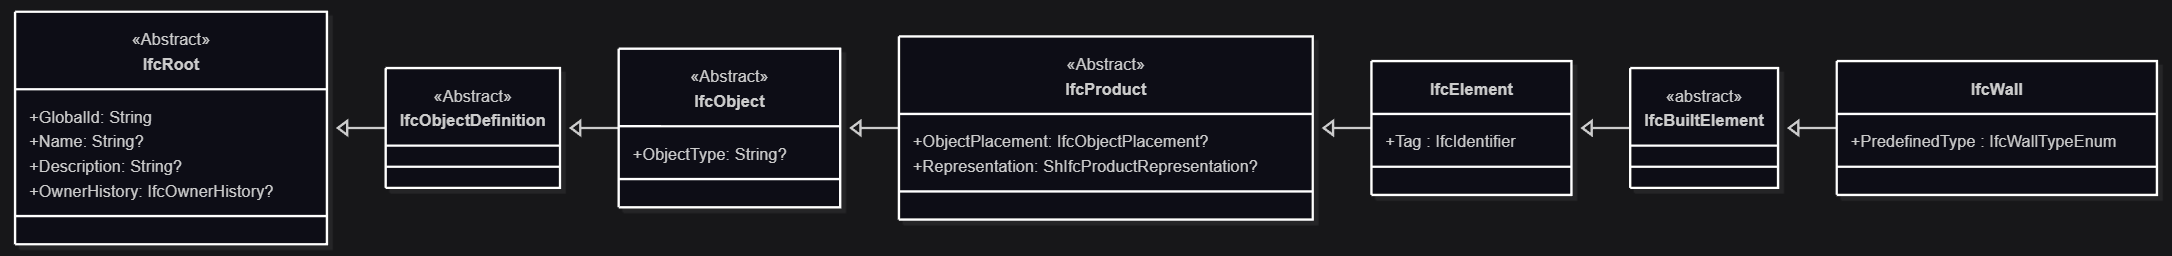
\includegraphics[width=1\textwidth]{IfcWallHierarchie.png} 
    \caption{Hierarchischer Aufbau der IFC-Klassen.}
    \label{fig:wall_hier}
\end{figure}

Die Objekte werden mittels Beziehung in Verbindung gebracht. Zum Beispiel hängt ein Gebäude (\textit{IfcBuilding}) mittels der Relation \textit{IfcRelAggregates}
an einem Bauplatz (\textit{IfcSite}). Als visuelles Beispiel soll folgende Grafik dienen:
\begin{figure}[H]
    \centering
    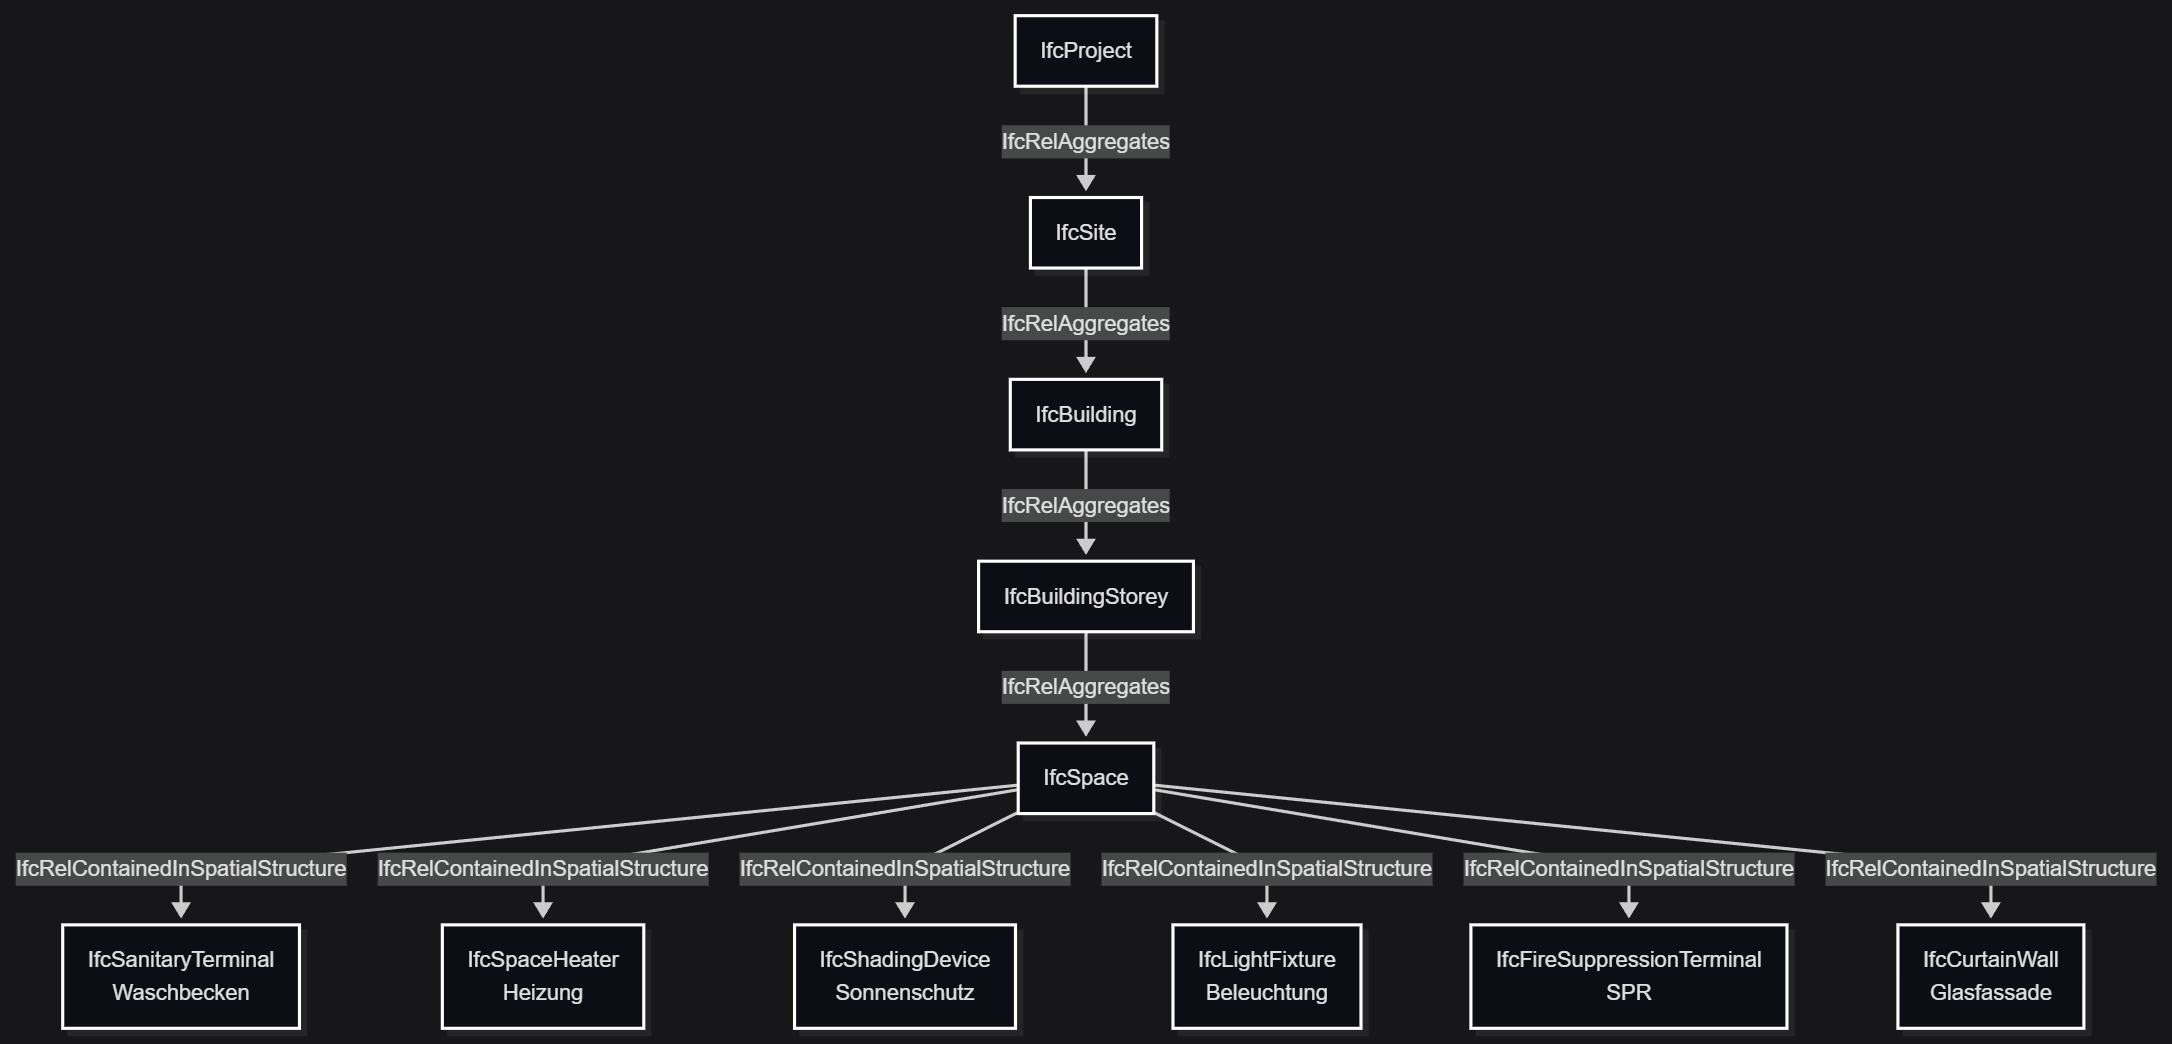
\includegraphics[width=1\textwidth]{LocationStructrue.png} 
    \caption{Struktueller Aufbau der IFC-Klassen.}
    \label{fig:loc_structure}
\end{figure}

\subsection{Graphdatenbanken}
Graphdatenbanken organisieren ihre Daten, wie der Name schon vermuten lässt, in Graphen. Das bedeutet Objekte werden als Knoten dargestellt, verbunden durch Kanten. Der große Vorteil hierbei ist die native Darstellung von Beziehungen zwischen den Objekten.
Dies wird insbesondere wichtig bei Datenmengen, bei welchen die Beziehungen zueinander ein elementarer Bestandteil der Datenerhebung darstellt. Bei den gängigsten Graphdatenbanken handelt es sich um sogenannte Labled Property Graphs. Hierbei können nicht nur
Knoten, sondern auch Kanten mit Labels und Eigenschaften versehen werden. 
\begin{figure}[htbp]
    \centering
    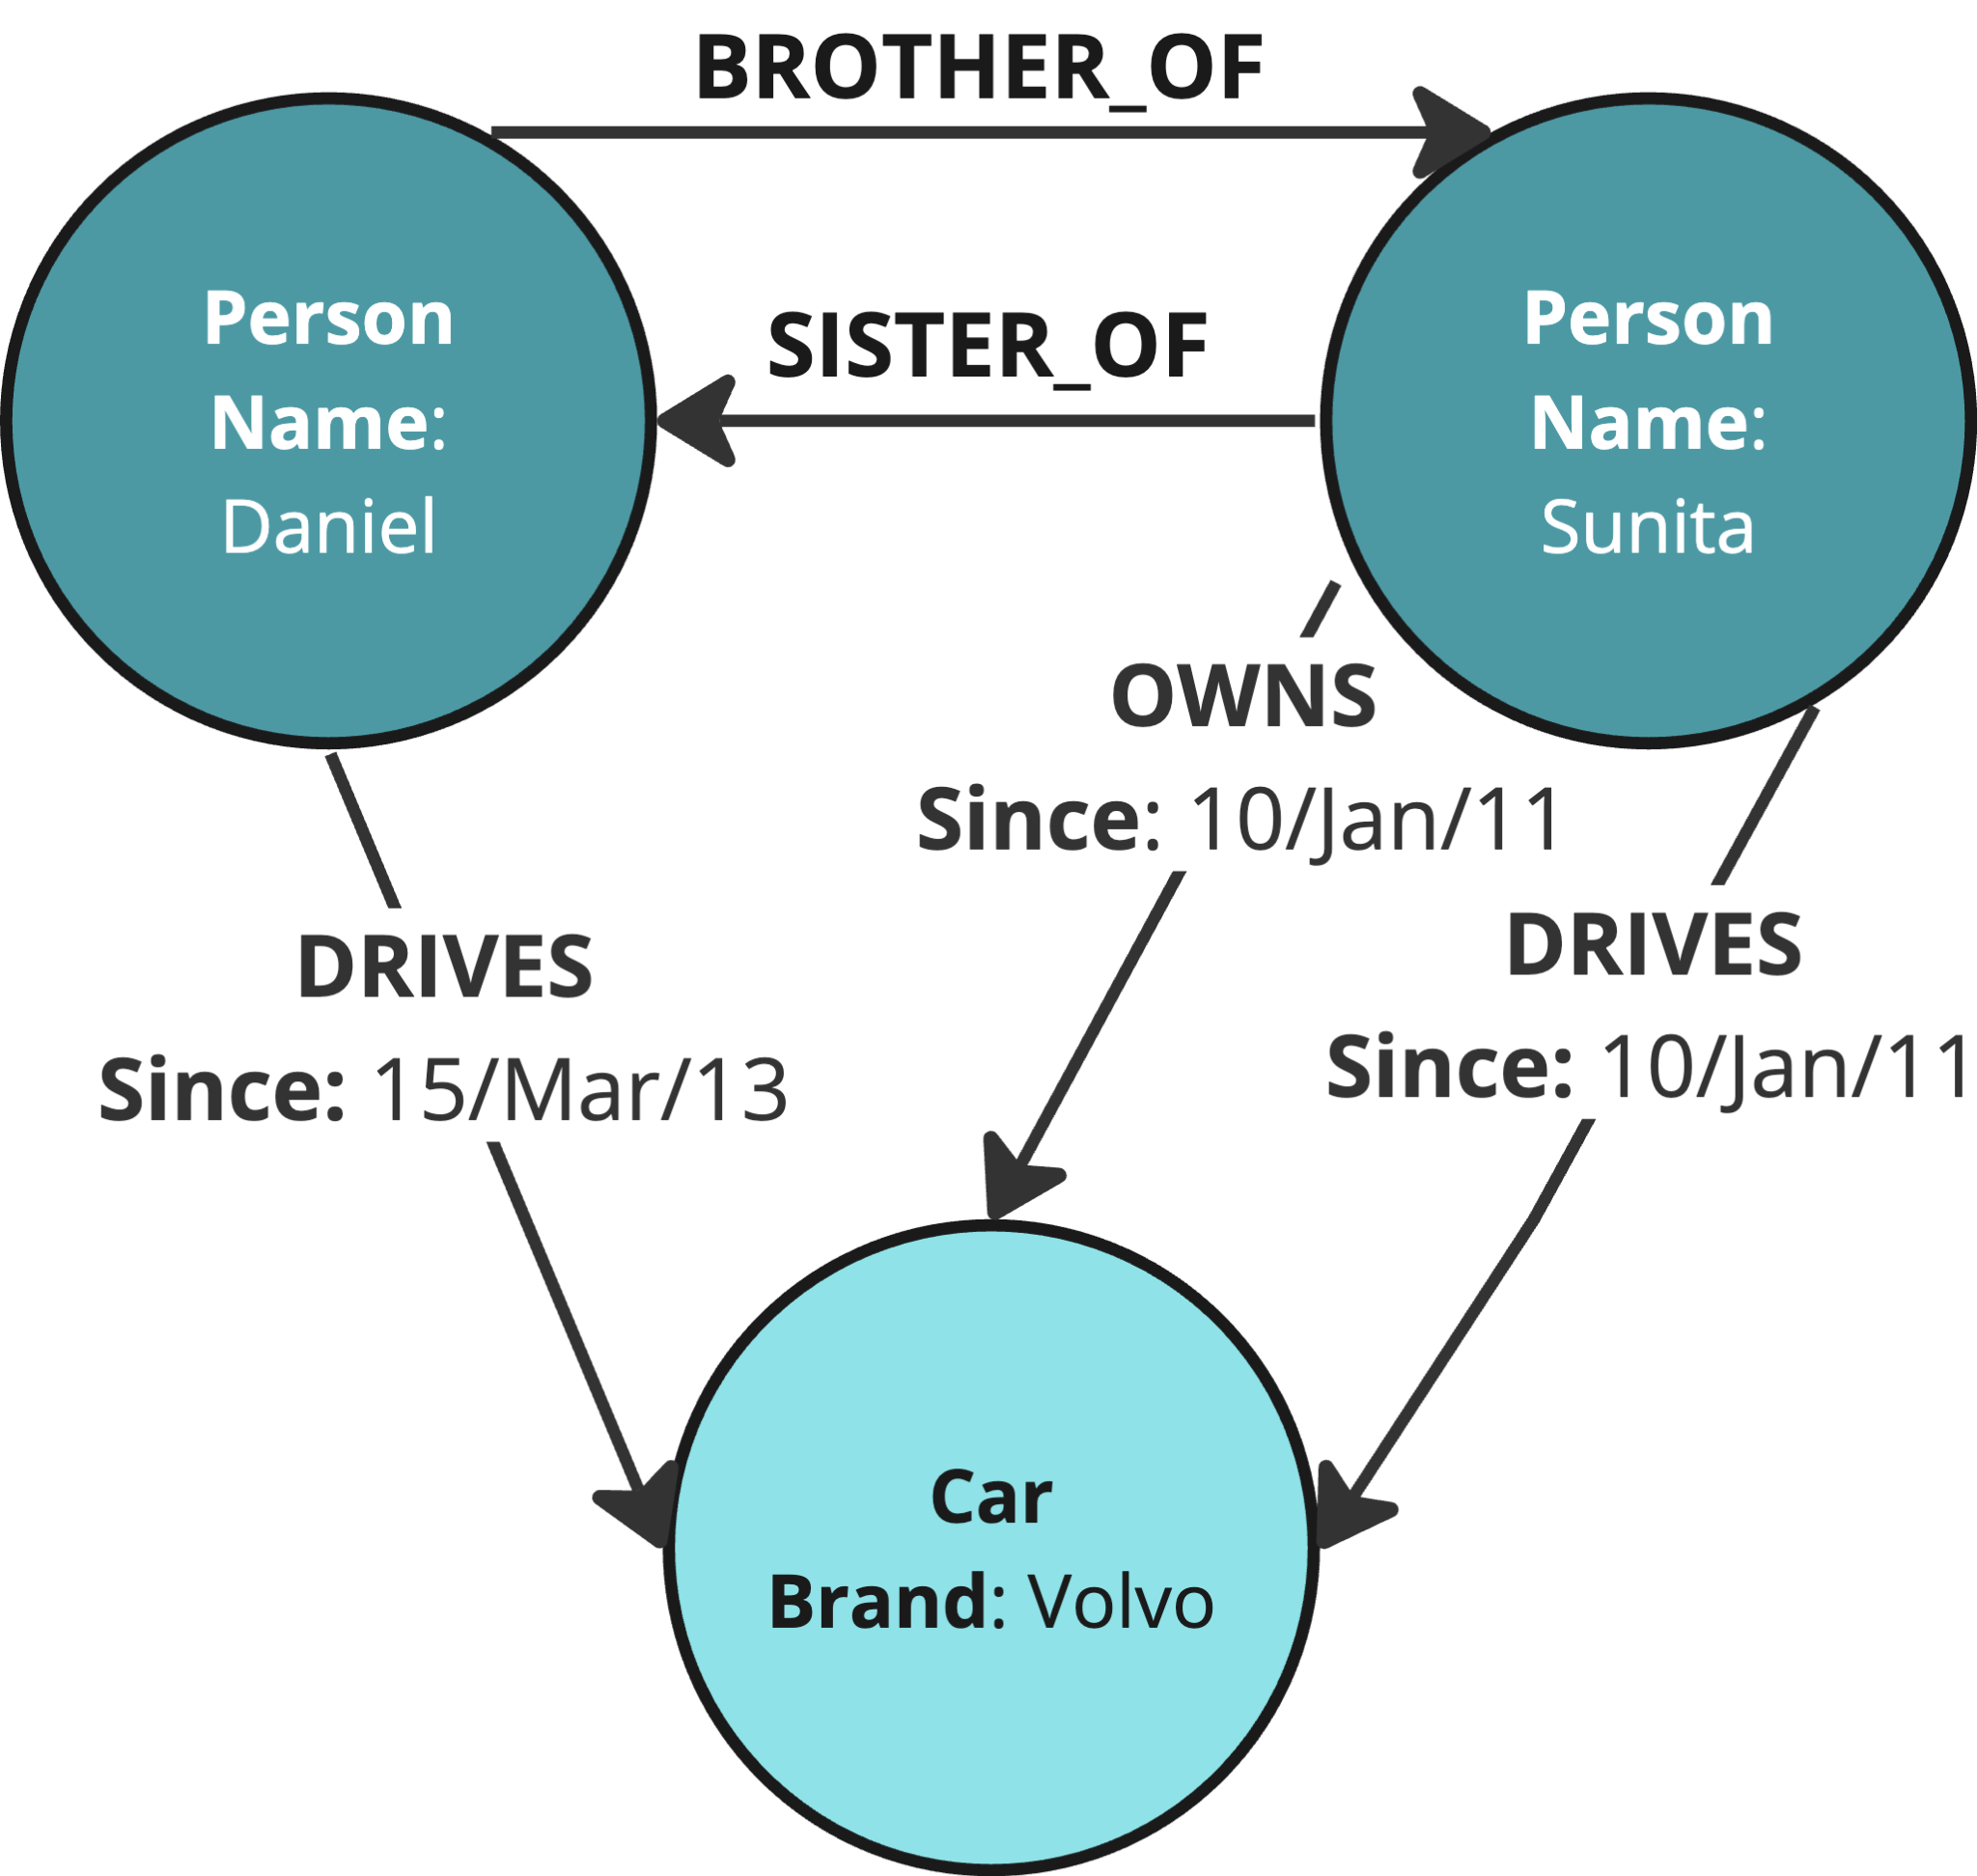
\includegraphics[width=0.5\textwidth]{property-graph.png} 
    \caption{Labled Property Graph \newline 
    (\url{https://dist.neo4j.com/wp-content/uploads/20240604025137/property-graph-model-1.png})}
    \label{fig:property_graph}
\end{figure}
Dieser Ansatz bietet eine hohe Flexibilität gegenüber relationalen Datenbanken, da hier der Datensatz logisch miteinander verknüpft werden kann und aufwände JOIN Operationen vermieden
werden können \cite{seidel2020graph}. Graphdatenbanken erfreuen sich vor allem großer Beliebtheit bei stark vernetzten Daten, wie Social Media, Betrugerkennung oder bei Lieferketten \cite{google_graphdb}, da hierbei der Analyse der Verbindungen im Vordergrund
steht.
%%TODO Eventuell Umschreiben (letzter Satz)
\subsubsection{neo4j}
Neo4j ist eine \gls{acid} konforme Graphdatenbank auf der Grundlage von Labled Property Graphs. Sie wurde erstmalig 2007 von Emil Eifrem veröffentlicht und avancierte zu einer der weltweit führenden Graphdatenbanken.

\subsubsection{GraphQL}
\subsection{Mircofrontends}
\subsection{Monorepos}
\newpage
\section{Graphbasiertes Datenmodell und Schnittstellendesign}
%% IFC Datenmodell sehr hierarchisch und vernetzt
%% in STEP Files organisiert
%% relationelle Datenbanken ungeignet weil Beziehungen nicht nativ, JOIN Operatoren notwenig -> aufwendug
%% realitätsnah und intuitive Darstellung der Daten
\subsection{Graphbasierte Domänenmodellierung für IFC-Daten}
\subsection{GraphQL als Vermittlungsinstanz}
%% Bessereres Wort als Vermittler irgendwas was die Kommunikation
%% stuert strukturiert und vereinfacht -> schema gibt typsicherheit
%% resolver können Daten effizient abfragen, Mutationen sichern revisionssicherheit etc.
\subsection{Das einheitliche API-Gateway: Datenabfrage via GraphQL}
%% Warum GraphQL geeignet ist als Vermittler
%% Was die Vorteile sind -> Schema, Typsicherheit
%% fest definierte allgemeine schnittstelle
%% Überleitung Frontend Vermittlungsschicht die mehr abstrahiert als Neo4js Cypher
%% Transparenz übergeifend
%% Revisionssicherheit durch Mutationen Schemas quasi Ground truth (Graphdatenbank) behalten
\newpage
% !TEX root = ../Abschlussarbeit_DE.tex
\section{Modulare Softwarearchitektur mittels Module Federation}
Jede Großbaustelle hat ihre eigenen individuellen Herausforderungen. Da jedoch viele Softwarelösungen als Allround-Lösungen konzipiert sind, 
scheitern sie oft an den spezifischen Detailanforderungen oder sind zu komplex und können so ihr Potenzial bei Weitem nicht ausschöpfen \cite[Kap.~3.1]{feth2023studie}. 
In der Praxis führt dies oft zu individuellen Spezialaufträgen an die Softwarehersteller - ein Prozess, der meist mit erheblichen Zusatzkosten und langen Entwicklungszeiten 
verbunden ist \cite[Kap.~4.1]{feth2023studie}. 
Um dem entgegenzuwirken, bedarf es einer flexiblen und vor allem einfach erweiterbaren Struktur, in welcher individuelle Softwarelösungen unkompliziert implementiert werden können. 
Ein möglicher Ansatzpunkt hierfür ist das Konzept der Microfrontends. Dabei werden einzelne Funktionalitäten als eigenständige Webapplikationen entwickelt, 
die sich zu einer gemeinsamen Benutzeroberfläche zusammenfügen lassen. 
%% Einzelne Gewerke können einfach hinzugefügt werden oder erp software
%% Vorteile gegenüber Monolithen (z.B. unabhängige Entwicklung und Deployment, skaliebarkeit, spezielle Lösungen)
%% Wichtige Dinge wie Kommunikation erwähnen 
\subsection{Aufbau von Microfrontends}
%% Aufbau (einzelne Komponenten wie z.B. Header )
%% Erklärung von Shell und Routing
\subsection{Kommunikation zwischen Microfrontends}
%% LocalStorage oder andere muss noch recherchiert ewrden
%% Nutzen von GraphQL mit listeners
\subsection{Konfiguration einer Microfrontendarchitektur}
%% Beispiel Vite
%% Erwähnung Monorepo
%% relativ straight forward wie gemacht wird
%% Shell Scripte
%% Konfigdatei für ports etc ver microfrontends
\newpage
% !TEX root = ../Abschlussarbeit_Jan_Händl.tex
\section{Verknüpfung der Microfrontends und der Graphdatenbank}
%% Allgemeine Anbindung
%% Erstellen eines prototyps zur veranschaulichung
%% GraphQL mit listeners
%% erwähnung von Middlewares
\subsection{Deployment Graphdatenbank}
\subsection{Multi-Tenant Fähigkeit}
%% konzentration auf App nicht auf die Datenbankstruktur
%% evtl GraphQL mit exten type und dann auth hinzufügen
%% evtl erwähnung vorgefertigter Apps 
%% evtl GraphQL
%
%\input{Inhalt/Material und Methoden}
\newpage
% !TEX root = ../Abschlussarbeit_Jan_Händl.tex
\section{Zusammenfassung und Fazit}

\newpage
% !TEX root = ../Abschlussarbeit_Jan_Händl.tex
\section{Ausblick}
Die Ausblicke und möglichen Weiterentwicklungsansätze sind in Bezug auf die Microfrontend-Architektur, als auch das Domänenmodell vielfältig.
An erster Stelle steht die vollständige Überführung des IFC-Standards in GraphQL Schemata. Wie bereits in Absatz \ref{sec:graphql} erörtert, gestaltet sich aufgrund der Komplexität des IFC-Standards
eine 1:1 Abbildung des IFC-Standards in GraphQL Schemata als äußerst aufwendig. Hier könnte entweder eine Abstraktion des IFC-Standards zielführend sein \cite{wolf_20206_graphql}, oder die Nutzung von
größeren Sprachmodellen zur automatisierten Überführung in GraphQL Schemata. Eng damit verbunden ist die Entwicklung eines leistungsfähigen IFC-Parsers. Ein solcher Parser ist notwendig, um IFC-Dateien effizient in die Graphdatenbank importieren zu können.
Zwar existieren in der Praxis bereits verschiedene Open-Source-Parser \cite{wolf:2025:ifc2graphql} zur Verarbeitung von IFC-Dateien, allerdings ist keiner dieser Ansätze auf die spezifischen Anforderungen dieses Forschungsthemas optimiert. Es bedürfe daher eine individuelle Lösung.
Auch in Bezug auf Multi-Tenancy ergeben sich weitere Forschungsansätze. Innerhalb dieser Arbeit wurde lediglich eine clientseitige Umsetzung
innerhalb der Microfrontend-Architektur erwähnt, während GraphQL mittels seiner @auth Direktive ein Rechtemanagement auf dem Server ermöglichen könnte. Dabei könnte der Nutzen und eine mögliche Umsetzung eines Rechtemanagements innerhalb
einer Graphdatenbank thematisiert werden, oder das Zusammenspiel mit einer relationalen Datenbank. Dabei könnte auch die Erstellung eines Rechtemanagements an sich, mit notwendigen Rollen und Berechtigungen im Kontext des Inbetriebnahmemanagements, als Forschungsthema dienen.
Neben diesen möglichen Ansätzen beinhaltet auch die Microfrontend-Architektur offene Fragen, wie beispielsweise eine durchgehende \ac{CI/CD}-Pipeline zur automatisierten Bereitstellung der einzelnen Microfrontends.
Hier könnten insbesondere die Herausforderungen des Bereitstellens und Komposition der einzelnen Microfrontends im Vordergrund stehen, sowie eine mögliche automatische Skalierung, um Lastspitzen auszugleichen. Analog zu klassischen Microservices könnte dies das Potential dieser verteilten Systeme weiter ausschöpfen. \\
Als weiterer wichtiger Punkt wären mögliche Implementierungen anderer Frontendtechnologien neben React zu nennen. Da Module Federation unabhängig von Frameworks ist, könnten eine Implementierung anderer Frontendtechnologien die Technologieunabhängigkeit weiter untermauern. Im Zuge dessen wäre auch die frameworkübergreifende Interaktion zwischen den Microfrontends, in Bezug auf Kommunikation, Routing und Isolation, von Interesse. \newline
Den größten Erkenntnisgewinn verspricht jedoch die Validierung des Gesamtsystems unter realitätsnahen Bedingungen. Ein empirisches Testen der Graphdatenbank mit großen IFC-Datenmengen sowie die gleichzeitige Nutzung der Microfrontends durch eine Vielzahl von Akteuren würde den größten Informationsgehalt hinsichtlich der tatsächlichen Performance, Skalierbarkeit, Effizienz und Systemstabilität liefern. Erst durch ein solches Last- und Stressszenario lässt sich die Praxistauglichkeit der entwickelten Microfrontend-Architektur in Verbindung mit dem graphbasierten Domänenmodell nachweisen.   % Dein eigentlicher Text

% --- 4. NACHSPANN ---
% !TEX root = ../Abschlussarbeit_Jan_Händl.tex
\thispagestyle{empty}
\addsec{Erklärung}
Hiermit erkläre ich, dass ich die vorgelegte Arbeit selbstständig verfasst, keine anderen als die
angegebenen Quellen und Hilfsmittel benutzt sowie alle wörtlich oder sinngemäß übernommenen
Stellen in der Arbeit als solche und durch Angabe der Quelle gekennzeichnet habe. Dies gilt auch für
Zeichnungen, Skizzen, bildliche Darstellungen, Quellen aus dem Internet sowie für im
Zusammenhang mit der Arbeit entstandene Produkte (z.B. Programmcode, Designentwürfe).\\
Ich versichere, dass ich mich generativer KI-Werkzeuge lediglich als Hilfsmittel bedient habe
und in der vorliegenden Arbeit mein gestalterischer Einfluss überwiegt. Unter der „Übersicht
verwendeter Hilfsmittel“ habe ich sämtliche verwendeten KI-Werkzeuge benannt
(Bezeichnung der Anwendung, URL, Seitenangabe damit erstellter Textpassagen). Ich habe
Textpassagen im Text, die KI-generierte Textpassagen durch ** gekennzeichnet (*KI generierte Textpassage*). Ich versichere, dass ich keine KI-Werkzeuge verwendet habe,
deren Nutzung der Prüfer / die Prüferin explizit in Textform ausgeschlossen hat.
\\
[4cm]
\noindent\rule{5cm}{.4pt}\hfill\rule{5cm}{.4pt}\par
\noindent Datum, Ort \hfill \autor \\

\newpage
\printglossaries
\clearpage
% !TEX root = ../Abschlussarbeit_Jan_Händl.tex
\appendix
\section{Anhang}

\subsection{Hilfsmittel}
\label{subsec:hilfsmittel}
Folgend werden die genutzten Hilfsmittel aufgelistet.
\begin{table}[H]
  \centering
  \renewcommand{\arraystretch}{1.4} % Mehr Zeilenabstand
  \setlength{\tabcolsep}{12pt}      % Mehr Spaltenabstand
  \caption{Hilfsmittel}
  \label{tab:hilfsmittel}
  \begin{tabularx}{\textwidth}{LLL}
    \toprule
    \textbf{Hilfsmittel}                                        & \textbf{Werkzeuge}                                                   & \textbf{Verwendung}                                      \\
    \midrule
    Zeichentool für Skizzen und Diagramme                       & Mermaid, Excalidraw, Screenshots                                     & Abb. 2.1, 2.2, 2.3, 2.4, 3.4, 4.1                        \\ \hline
    Rechtschreib- und Grammatikprüfung                          & Gemini 3.5, LTeX+ grammar/spell checking using LanguageTool  v15.7.1 & Komplette Arbeit                                         \\ \hline
    Schreibprogramm                                             & Visual Studio Code, LaTeX Workshop                                   & Komplette Arbeit                                         \\ \hline
    Version Control System                                      & Git                                                                  & Komplette Arbeit                                         \\ \hline
    Literaturrecherche                                          & Google Scholar, Researchgate, NotebookLM                             & Komplette Arbeit                                         \\ \hline
    Integrated Development Environment                          & Visual Studio Code                                                   & Programmierteil (siehe USB-Stick)                        \\ \hline
    Deployment Neo4j Datenbank                                  & Docker Compose                                                       & Programmierteil (siehe USB-Stick)                        \\ \hline
    Visualisierung Neo4j Graph                                  & Neo4j Browser                                                        & Abb. 3.1, 3.2, 3.4                                       \\ \hline
    Generierung Code und GraphQL Schema, Resolver und Mutations & Gemini 3.1, Gemini 3.5                                               & Programmierteil (siehe USB-Stick), Listing. 6, 8, 10, 11 \\ \hline
    Konfiguration Latex Projekt                                 & Gemini 3.1, Gemini 3.5                                               & Komplette Arbeit                                         \\

    \bottomrule
  \end{tabularx}
\end{table}

\subsection{Verwendete KI-Prompts}
\label{subsec:ki_prompts}
Folgend sind die maßgeblichen KI-Prompts für die Arbeit aufgelistet.
\begin{table}[H]
  \centering
  \renewcommand{\arraystretch}{1.4} % Mehr Zeilenabstand
  \setlength{\tabcolsep}{12pt}      % Mehr Spaltenabstand
  \caption{Verwendete KI-Prompts}
  \label{tab:ki_prompts}
  \begin{tabular}{lll}
    \toprule
    \textbf{Prompt}        & \textbf{Ergebnis}             & \textbf{KI Modell}     \\
    \midrule
    Formuliere den Text um & Vorschläge für Formulierungen & Gemini 3.5, Gemini 3.1 \\
    \bottomrule
  \end{tabular}
\end{table}

\subsection{Routing in Microfrontends}
\label{subsec:microfrontends_routing}
In diesem Abschnitt wird der exemplarische Vergleich zwischen dem URL-basierten Routing und einem zustandsbasierten Routing (SPA) dargestellt.
\begin{lstlisting}[language=Javascript, caption={Exemplarischer Vergleich zwischen Url Routing und einer SPA}, label={lst:microfrontends_routing}]
import React, { useState } from 'react';
import { BrowserRouter, Routes, Route, Link } from 'react-router-dom';
// 1. Komponenten für das State-basierte Routing (SPA)
const RoombookApp = React.lazy(() =>
  import("roombook/RoombookApp").catch(() => {
    return {
      default: () => (
        <div className="p-8 text-center text-destructive bg-destructive/10 rounded-xl m-8">
          Fehler beim Laden von Roombook! Ist die Remote App (Port 5174)
          gestartet?
        </div>
      ),
    };
  }),
);
const InsightsApp = React.lazy(() =>
  import("insights/InsightsApp").catch(() => {
    return {
      default: () => (
        <div className="p-8 text-center text-destructive bg-destructive/10 rounded-xl m-8">
          Fehler beim Laden von Insights! Ist die Remote App (Port 5175)
          gestartet?
        </div>
      ),
    };
  }),
);
// 2. Komponenten für das URL-basierte Routing
const RoombookApp = () => <p>Komponente: RoombookApp (URL)</p>;
const InsightsApp = () => <p>Komponente: InsightsApp (URL)</p>;
export default function RoutingVergleichApp() {
  // State für das zustandsbasierte Umschalten
  const [activeTab, setActiveTab] = useState('A');
  return (
    <BrowserRouter>
      {/* MECHANISMUS 1: URL-BASIERTES ROUTING (Ändert die Browser-URL)*/}
      <div>
        <h3>1. URL-basiertes Routing</h3>
        <nav>
          <Link to="/roombookapp"/>
          <Link to="/insightsapp"/>
        </nav>

        <Routes>
          <Route path="/roombookapp" element={<RoombookApp />} />
          <Route path="/insightsapp" element={<InsightsApp />} />
        </Routes>
      </div>
      <hr />
      {/*MECHANISMUS 2: STATE-BASIERTES ROUTING (SPA)*/}
      <div>
        <h3>2. State-basiertes Routing</h3>
        <nav>
          <button onClick={() => setActiveTab('A')}>Zeige RoombookApp</button>
          <button onClick={() => setActiveTab('B')}>Zeige InsightsApp</button>
        </nav>
        <div>
          {activeTab === 'A' && <RoombookApp />}
          {activeTab === 'B' && <InsightsApp />}
        </div>
      </div>
    </BrowserRouter>
  );
}
\end{lstlisting}

\subsection{Cypher-Datenbankabfragen}
\label{subsec:cypher_abfragen}
Folgend wird ein exemplarisches Cypher-Statement aufgeführt, welches zur Abfrage von Sensorbeziehungen in der Neo4j-Graphdatenbank verwendet wird.
\begin{lstlisting}[language=cypher, caption={Exemplarische Cypher-Abfrage für aktive Sensoren in einem Raum}, label={lst:cypher_active_sensors}]
MATCH (r:Room {number: "1.04"})<-[:LOCATED_IN]-(s:Sensor)
WHERE s.status = "ACTIVE"
RETURN r, s;
\end{lstlisting}

\subsection{Ergänzende Diagramme und Daten}
\label{subsec:ergaenzende_diagramme}
Hier können weitere unterstützende Diagramme wie UML-Klassendiagramme, Flussdiagramme oder zusätzliche Messdaten eingefügt werden, die den Rahmen des Hauptteils sprengen würden.
Beispielsweise zeigt ein Systemarchitektur-Diagramm die Interaktion zwischen den Microfrontends und dem API-Gateway über GraphQL.
\begin{center}
  \textit{[Hier kann ein zusätzliches Architekturdiagramm oder Flussdiagramm eingefügt werden]}
\end{center}

\bibliographystyle{unsrt} % 'unsrt' sortiert nach Erscheinen im Text (Standard für IT)
\bibliography{Bibliographie} % Ohne die Endung .bib

\end{document}